\graphicspath{{images/}}

\section*{Turingmaschinen}

\begin{theorem}{Turingmaschinen (TM)}
    \begin{itemize}
        \item Einen Lese- / Schreib-Kopf
        \item Ein unendliches Band von Zellen
      \end{itemize}
      
      Eine deterministischer Turing-Maschine TM ist ein 7-Tupel
      $$
      M=\left(Q, \Sigma, \Gamma, \delta, q_{0}, \sqcup , F\right)
      $$
      \begin{itemize}
        \item Menge von Zuständen: $Q$
        \item Alphabet der Eingabe: $\Sigma$
        \item Bandalphabet: $\Gamma$ und $\Sigma \subset \Gamma$
        \item Übergangsfunktion: $\boldsymbol{\delta}: \boldsymbol{Q} \times \boldsymbol{\Gamma} \rightarrow \boldsymbol{Q} \times \boldsymbol{\Gamma} \times \boldsymbol{D}, \boldsymbol{D}=\{\boldsymbol{L}, \boldsymbol{R}\}$
        \item Anfangszustand: $q_{0} \in Q$
        \item Akzeptierende Zustände: $F \subseteq Q$
        \item Leerzeichen ${ }_{\sqcup }$, mit ${ }_{\mu} \in \Gamma$ und ${ }_{\mu} \notin \Sigma$
      \end{itemize}
      Sie bildet das 2-Tupel $(q, X)$ auf das Tripel $(p, Y, D)$

    \begin{itemize}
    \item $q, p \in Q$ und $X, Y \in \Gamma$
    \item $D=$ Direction
    \item $X=$ Read
    \item $Y=$ Overwrite
    \end{itemize}
    $$
    q-X / Y, D \rightarrow p
    $$
\end{theorem}

\begin{definition}{Band}
    \begin{itemize}
        \item Unterteilt in einzelne Zellen mit jeweils einem beliebigen Symbol
        \item Beinhaltet zu Beginn die Eingabe, d.h. ein endliches Wort aus $\Sigma^{*}$. Alle anderen Zellen enthalten das besondere Symbol 4 .
    \end{itemize}
\end{definition}

\begin{definition}{Konfiguration}
    einer Turing-Maschine $M$ ist durch die folgenden Angaben eindeutig spezifiziert
    \begin{itemize}
    \item Zustand der Zustandssteuerung
    \item Position des Lese- / Schreibkopfes
    \item Bandinhalt
    \end{itemize}
\end{definition}

\begin{concept}{Semi-Unendliches Band}\\
    Das Band der Turingmaschine ist nur in eine Richtung unendlich.\\
    Jede Sprache $L$ die von einer TM $T$ akzeptiert wird, wird auch von einer TM mit semi-unendlichem Band akzeptiert.\\
    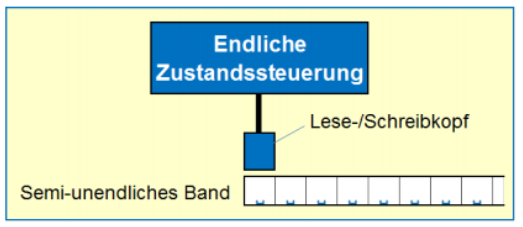
\includegraphics[width=0.3\linewidth]{semi_unendliches_band.png}
\end{concept}

\begin{concept}{Mehrere Stacks}\\
    Jede Sprache $L$ die von einer TM $T$ akzeptiert wird, wird auch von einer 2Stack-Maschine $S$ akzeptiert.\\
    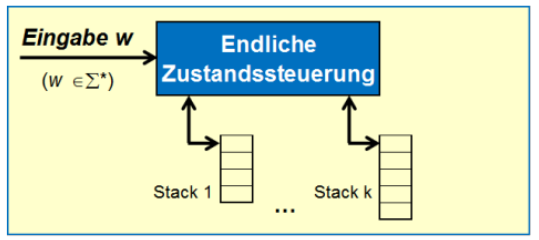
\includegraphics[width=0.3\linewidth]{mehrere_stacks_tm.png}
\end{concept}

\begin{concept}{Zähler-Maschinen}\\
    Eine Zähler-Maschine (Counter Machine) mit $k$ Zählern entspricht einer $k$ Stack-Maschine mit dem Unterschied, dass die Stacks durch einfache Zähler ersetzt werden.\\
    Jede Sprache $L$ die von einer TM $T$ akzeptiert wird, wird auch von einer 2Zähler-Maschine $Z$ mit 2 Zählern akzeptiert.\\
    \includegraphics[width=0.3\linewidth]{zähler_maschinen.png}
\end{concept}

\begin{concept}{TM mit Speicher}\\
    In der endlichen Zustandssteuerung einer TM können ausser dem SteuerZustand zusätzlich endlich viele Daten-Zustände gespeichert werden.\\
    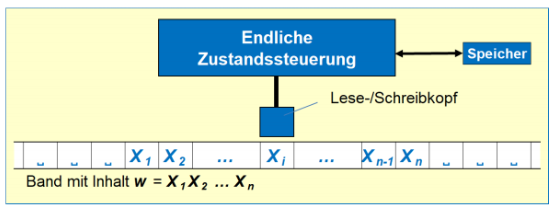
\includegraphics[width=0.3\linewidth]{tm_mit_speicher.png}
\end{concept}

\begin{concept}{Mehrere Spuren}
    \begin{itemize}
        \item Das Band der TM setzt sich aus mehreren «Spuren» zusammen.
        \item Jede Spur kann ein Symbol des Bandalphabets speichern.
    \end{itemize}
    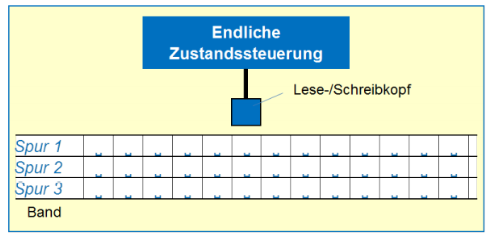
\includegraphics[width=0.3\linewidth]{mehrere_spuren.png}
\end{concept}

\begin{concept}{Mehrere Bänder}
    \begin{itemize}
        \item TM mit endlich vielen Bändern und Lese- / Schreibköpfen
        \item Jeder Lese- / Schreibkopf kann unabhängig auf ein Band zugreifen
    \end{itemize}
    \includegraphics[width=0.3\linewidth]{mehrere_bänder.png}
\end{concept}

\begin{example2}{Mehrband-Maschine}\\
    Spezifizieren Sie eine TM $M_{4}$, welche die Subtraktion von zwei natürlichen Zahlen $(a-b$, mit $a \geq b)$ realisiert.\\
    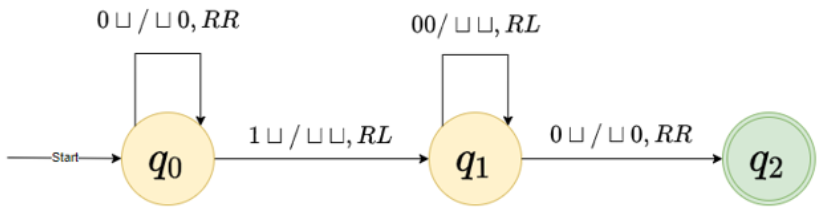
\includegraphics[width=0.5\linewidth]{mehrband_maschine1.png}\\
    Beispiel: $4-2=2$\\
    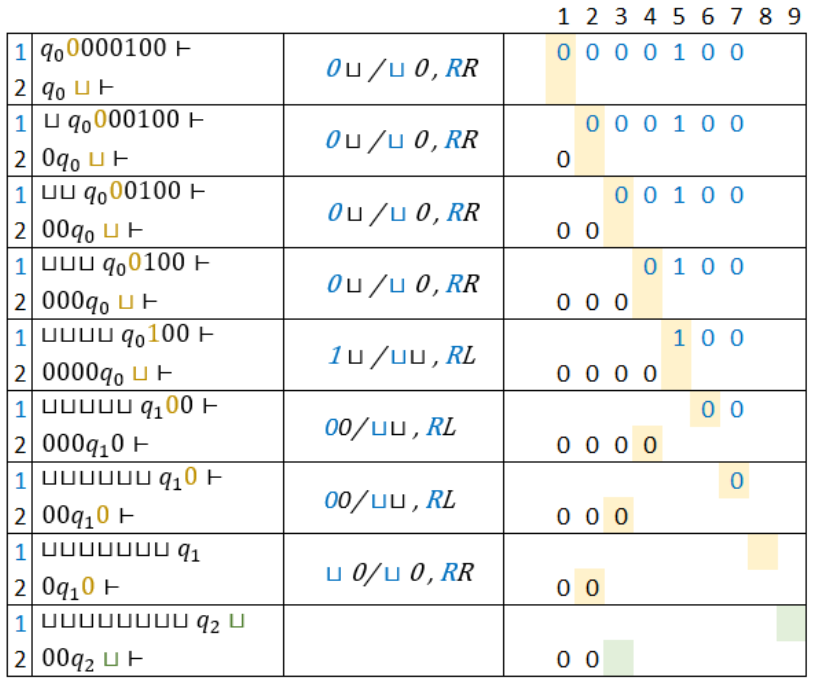
\includegraphics[width=1\linewidth]{mehrband_maschine2.png}
\end{example2}